\ifthenelse{\equal{\lang}{en}}{
\section{Books Studied}

\bookCard
    {\bookCover{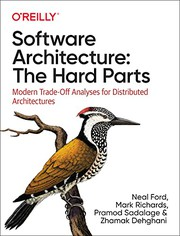
\includegraphics[width=15mm]{img/books/hard_parts.jpg}}}
    {Software Architecture: The Hard Parts}
    {450p -- Hard}
    {\fivestars}
    {N. Ford, M. Richards, P. Sadalage \& Z. Dehghani}
    {04/2026 -- ongoing}
    {Software architecture's "axioms" constantly shift with the ecosystem, so architects must continually question assumptions and weigh trade-offs rather than trust fixed rules.}
    {It filled a gap I had in how to measure and optimize software systems: every decision is a trade-off. Sometimes you fall in love with a technology and forget there's no universal solution for every problem -- each problem usually needs a set of frameworks aligned with the business requirements.}

\bookCard
    {\bookCover{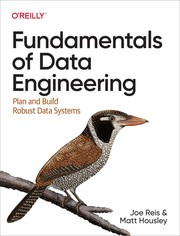
\includegraphics[width=15mm]{img/books/data_engineering.jpg}}}
    {Fundamentals of Data Engineering}
    {~400p -- Hard}
    {\fivestars}
    {Joe Reis \& Matt Housley}
    {08/2026}
    {Data engineering is the lifecycle discipline (generation, storage, ingestion, transformation, serving) that turns raw data into reliable information for downstream teams.}
    {An incredible book on data engineering. Before it I confused different messaging systems with each other; it covers monitoring, traceability, and how to build a robust system. It sparked my interest in data architecture. It took me a lot of time and effort to finish, but I ended up applying everything I learned. A wonderful book.}

\bookCard
    {\bookCover{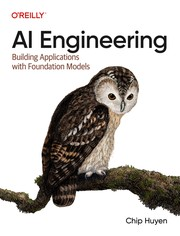
\includegraphics[width=15mm]{img/books/ai_engineering.jpg}}}
    {AI Engineering}
    {350p -- Hard}
    {\fivestars}
    {Chip Huyen}
    {04/2026}
    {Foundation models turned AI development from training custom models into "AI engineering" -- adapting general-purpose models via prompting, RAG and finetuning.}
    {This one also took me a lot of time and effort to finish, but I loved it too. It takes a different approach from traditional machine learning: it focuses on the infrastructure around AI models -- observability, monitoring, data drift -- a whole set of new problems that don't come up in the traditional software approach. It also explores the full lifecycle of AI products. What I loved most were LoRA adapters, which is actually the reason I got hired at Meduzia. A very complete book, highly recommended.}

\bookCard
    {\bookCover{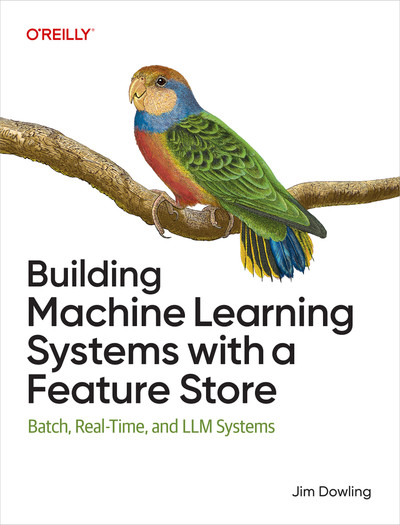
\includegraphics[width=15mm]{img/books/feature_store.jpg}}}
    {Building ML Systems with a Feature Store}
    {492p -- Hard}
    {\fivestars}
    {Jim Dowling}
    {03/2026}
    {ML and LLM systems should be organized as modular Feature/Training/Inference pipelines connected via a feature store, unifying batch, real-time and RAG architectures.}
    {A lot of fun -- I implemented a real-time system using a feature store, which is basically a shared space for models, data and resources across data scientists. It's fundamentally a data engineering book: it closes the gap between ML engineer and data engineer. What blew my mind was the organized way of solving problems -- before reading it, every step felt confusing, and this is where I learned the lifecycle of machine learning products (classic and LLM-based). It's a practical, very fun book. I also learned about data lineage: auditing a dataset from creation to consumption -- e.g. whether it passed through a database and what transformation was applied. It's the operationalization of a complex problem into data pipelines that are always the same -- that's what changed my way of thinking the most.}
}{
\section{Libros Estudiados}

\bookCard
    {\bookCover{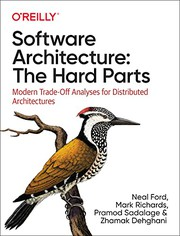
\includegraphics[width=15mm]{img/books/hard_parts.jpg}}}
    {Software Architecture: The Hard Parts}
    {450p -- Difícil}
    {\fivestars}
    {N. Ford, M. Richards, P. Sadalage y Z. Dehghani}
    {04/2026 -- en curso}
    {Los "axiomas" de la arquitectura de software cambian constantemente con el ecosistema, por lo que hay que cuestionar los supuestos y ponderar trade-offs en vez de reglas fijas.}
    {Llenó mi gap que tenía en cómo medir y optimizar sistemas de software: todas las decisiones son un balance. A veces uno se enamora de una tecnología y se olvida que no existe solución universal para todos los problemas -- cada problema suele requerir un conjunto de frameworks alineados siempre con los requerimientos del negocio.}

\bookCard
    {\bookCover{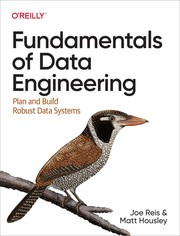
\includegraphics[width=15mm]{img/books/data_engineering.jpg}}}
    {Fundamentals of Data Engineering}
    {~400p -- Difícil}
    {\fivestars}
    {Joe Reis y Matt Housley}
    {08/2026}
    {La ingeniería de datos es la disciplina del ciclo de vida (generación, almacenamiento, ingesta, transformación, servido) que convierte datos crudos en información confiable.}
    {Libro increíble sobre data engineering. Antes del libro tenía una confusión entre distintos sistemas de mensajería; el libro habla de monitoreo, trazabilidad, cómo construir un sistema robusto. Este libro despertó mi interés en arquitectura de datos. Me costó mucho tiempo y esfuerzo completarlo, pero todo lo aprendido lo terminé aplicando. Libro maravilloso.}

\bookCard
    {\bookCover{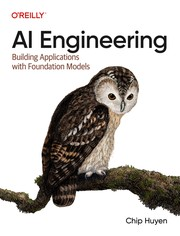
\includegraphics[width=15mm]{img/books/ai_engineering.jpg}}}
    {AI Engineering}
    {350p -- Difícil}
    {\fivestars}
    {Chip Huyen}
    {04/2026}
    {Los foundation models transformaron el desarrollo de IA: de entrenar modelos propios a hacer "AI engineering" -- adaptar modelos generales vía prompting, RAG y finetuning.}
    {Este libro también me costó mucho tiempo y esfuerzo terminar, pero también me encantó. Tiene un enfoque diferente al tradicional de machine learning: se centra en la infraestructura que acompaña a los modelos de IA (observabilidad, monitoreo, data drift), problemas nuevos que no surgían en el enfoque de software tradicional. También explora el ciclo de vida completo de productos de IA. Lo que más me encantó fueron los adaptadores LoRA, que de hecho fue la razón por la cual me contrataron en Meduzia. Libro muy completo, muy recomendado.}

\bookCard
    {\bookCover{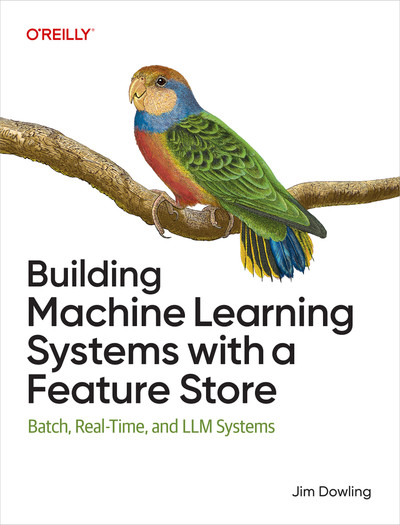
\includegraphics[width=15mm]{img/books/feature_store.jpg}}}
    {Building ML Systems with a Feature Store}
    {492p -- Difícil}
    {\fivestars}
    {Jim Dowling}
    {03/2026}
    {Los sistemas de ML y LLMs deberían organizarse como pipelines modulares de Feature/Training/Inference conectados por un feature store, unificando arquitecturas batch, real-time y RAG.}
    {Fue un libro muy divertido, donde implementé un sistema en tiempo real utilizando un feature store, que básicamente es un espacio para compartir modelos, datos y recursos entre científicos de datos. Es un libro fundamentalmente de data engineering: cierra el gap entre ML engineer y data engineer. Lo que me voló la cabeza es la forma organizada de resolver problemas -- antes de leerlo todos los pasos eran confusos, y aquí aprendí cómo es el ciclo de vida de productos de machine learning (clásicos y LLMs). Es un libro práctico, muy divertido. Otra cosa que aprendí es sobre el lineage de los datos: poder hacer una auditoría desde la creación hasta el consumo de los datasets, por ejemplo si pasó por una base de datos y qué transformación se le hizo. Es la operacionalización de un problema complejo en pipelines de datos que siempre son lo mismo -- lo que más me cambió la forma de pensar.}
}
